\subsection{Instrumentation Amplifier}\label{ssec:instrumentation-amplifier}

	\subsubsection{The Operational Amplifier}\label{sssec:operational-amplifier}

		A Operational Amplifier can be defined as a voltage amplifier with a differential input and a single-ended output. Operational Amplifiers are usually refered just as \textit{OPAMPs}. Thoose devices are largely used in eletronic circuits, theoretically they have infinite input impedance and infinite gain, this means that OpAmps do not drain current from the signals they are amplifying and they can amplify this signals with any gain \cite{mancini2003op}. Figure \ref{fig:opamp} shows the schematic symbol of the OpAmp.

	\begin{figure}[htbp]
		\centering
			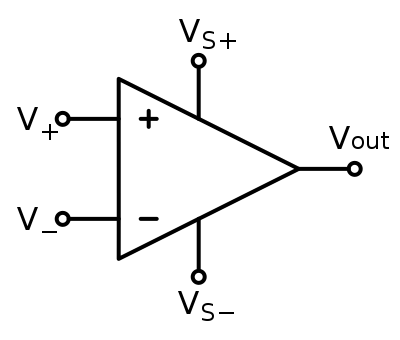
\includegraphics[scale=0.6]{figuras/fig-opamp.png}
		\caption{Operational Amplifier \cite{fig-opamp}}
		\label{fig:opamp}
	\end{figure}

	$V_{+}$ and $V_{-}$ are the OpAmp inputs, $V_{S+}$ and $V_{S-}$ are the power supply inputs. The voltage output $V_{out}$ is limited to the voltage values given by the power supply inputs. The gain of a operation amplifier can vary according to it's configuration, only the configuration relevant to this paper will be explained.

	\subsubsection{The Closed-loop amplifier}\label{ssec:closed-loop-amplifier}

		This may be the most common configuration for the operational amplifier.
		
	\begin{figure}[htbp]
		\centering
			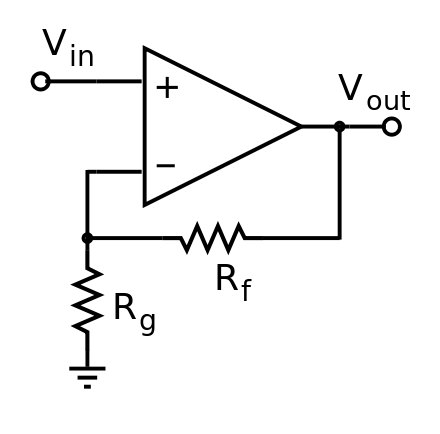
\includegraphics[scale=0.6]{figuras/fig-closed-loop-opamp.png}
		\caption{Operational Amplifier \cite{fig-closed-loop-opamp}}
		\label{fig:closed-loop-opamp}
	\end{figure}

		The output voltage of this amplifier is given by Equation \ref{eqn:gain-neg-closed-loop-amp} \cite{dorf-non-inverting-opamp-eqn}.

	\begin{equation}
		Vout =  \left( 1 + \frac{R_{f}}{R_{g}} \right) \cdot V_{in}
	\end{equation}\label{eqn-gain-neg-closed-loop-amp}

		The disadvantage of this OpAmp configuration is that only gains greater than one are achievable, in electronic instrumentation this is not a common issue because in this field of electronic engineering amplification is usually done to increase the resolution of signals, not to reduce it.

	\subsubsection{The Instrumentation Amplifier}\label{sssec:instrumentation-amplifier}

	In general, sensors and tranducers have very low voltage output levels (specially passive transducers), and therefore an amplification is fundamental. The most commonly used amplifier circuit in instrumentation engineering is the common joint differential amplifier more commonly refered as \textit{Instrumentation Amplifier} (Figure \ref{fig:instrumentation-amplifier}), which is very stable and significantly reduces the output signal noise \cite{wait1975introduction}.

	\begin{figure}[htbp]
		\centering
			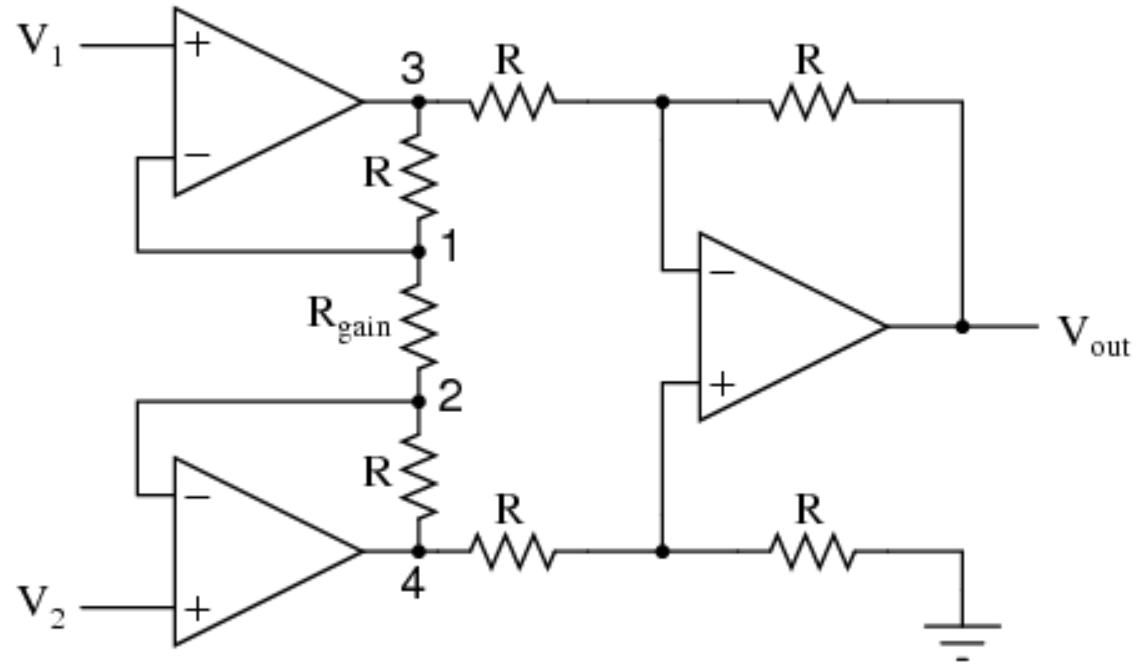
\includegraphics[scale=1.25]{figuras/fig-instrumentation-amp.png}
		\caption{Instrumentation Amplifier \cite{3opamp}}
		\label{fig:instrumentation-amplifier}
	\end{figure}

	The instrumentation amplifier has two stages, the first stage consists in amplifying both inputs of a sensor, with the gain of this amplification stage controlled by $R_{gain}$ in Figure \ref{fig:instrumentation-amplifier}. The second stage consists in taking the difference of the two input signals. If the differentiation happens before the amplification, noise may be so big in the input signals that some signal information might be lost. In the instrumentation amplifier noise and signal is amplified on the first stage, considering that the noise is similar in both inputs the differential stage will take out the noise and only output the difference between both inputs. One advantage of this amplifier is that it has high input impedances, that means it will not drain significant current from the signal, i.e., it will not interfere with the measure \cite{thomsen2003application}. Another advantage is that the gain of this amplifier can be adjusted with just one resistor \cite{mettingvanrijn1994amplifiers}.
	\par
	The gain of the instrumentation amplifier is given by the following \ref{eqn:gain-instrumentationAmplifier} \cite{analogDevDesignersGuide}.

	\begin{equation}
		Vout = \left( V_{2} - V_{1} \right) \cdot \left( 1 + \frac{2\cdot R}{R_{gain}} \right)
	\end{equation}\label{eqn:gain-instrumentationAmplifier}

	Something interesting to notice is that if we take out the $R_{gain}$ (open load), the gain of the amplifier is equal to one. Besides this advantageous behavor of the instrumentation amplifier, it is quite hard to make it work with seven resistors and three operation amplifiers because of components imprecision. Hence, it is more practical to work with ICs that ensure the symmetry of between those components. As an example, there is the Texas Instruments INA118 \cite{ina118}, which is one of many encapsulated solutions for the instrumentation amplifier, the schematic of this component is shown in Figure \ref{fig:ina118}.

	\begin{figure}[htbp]
		\centering
			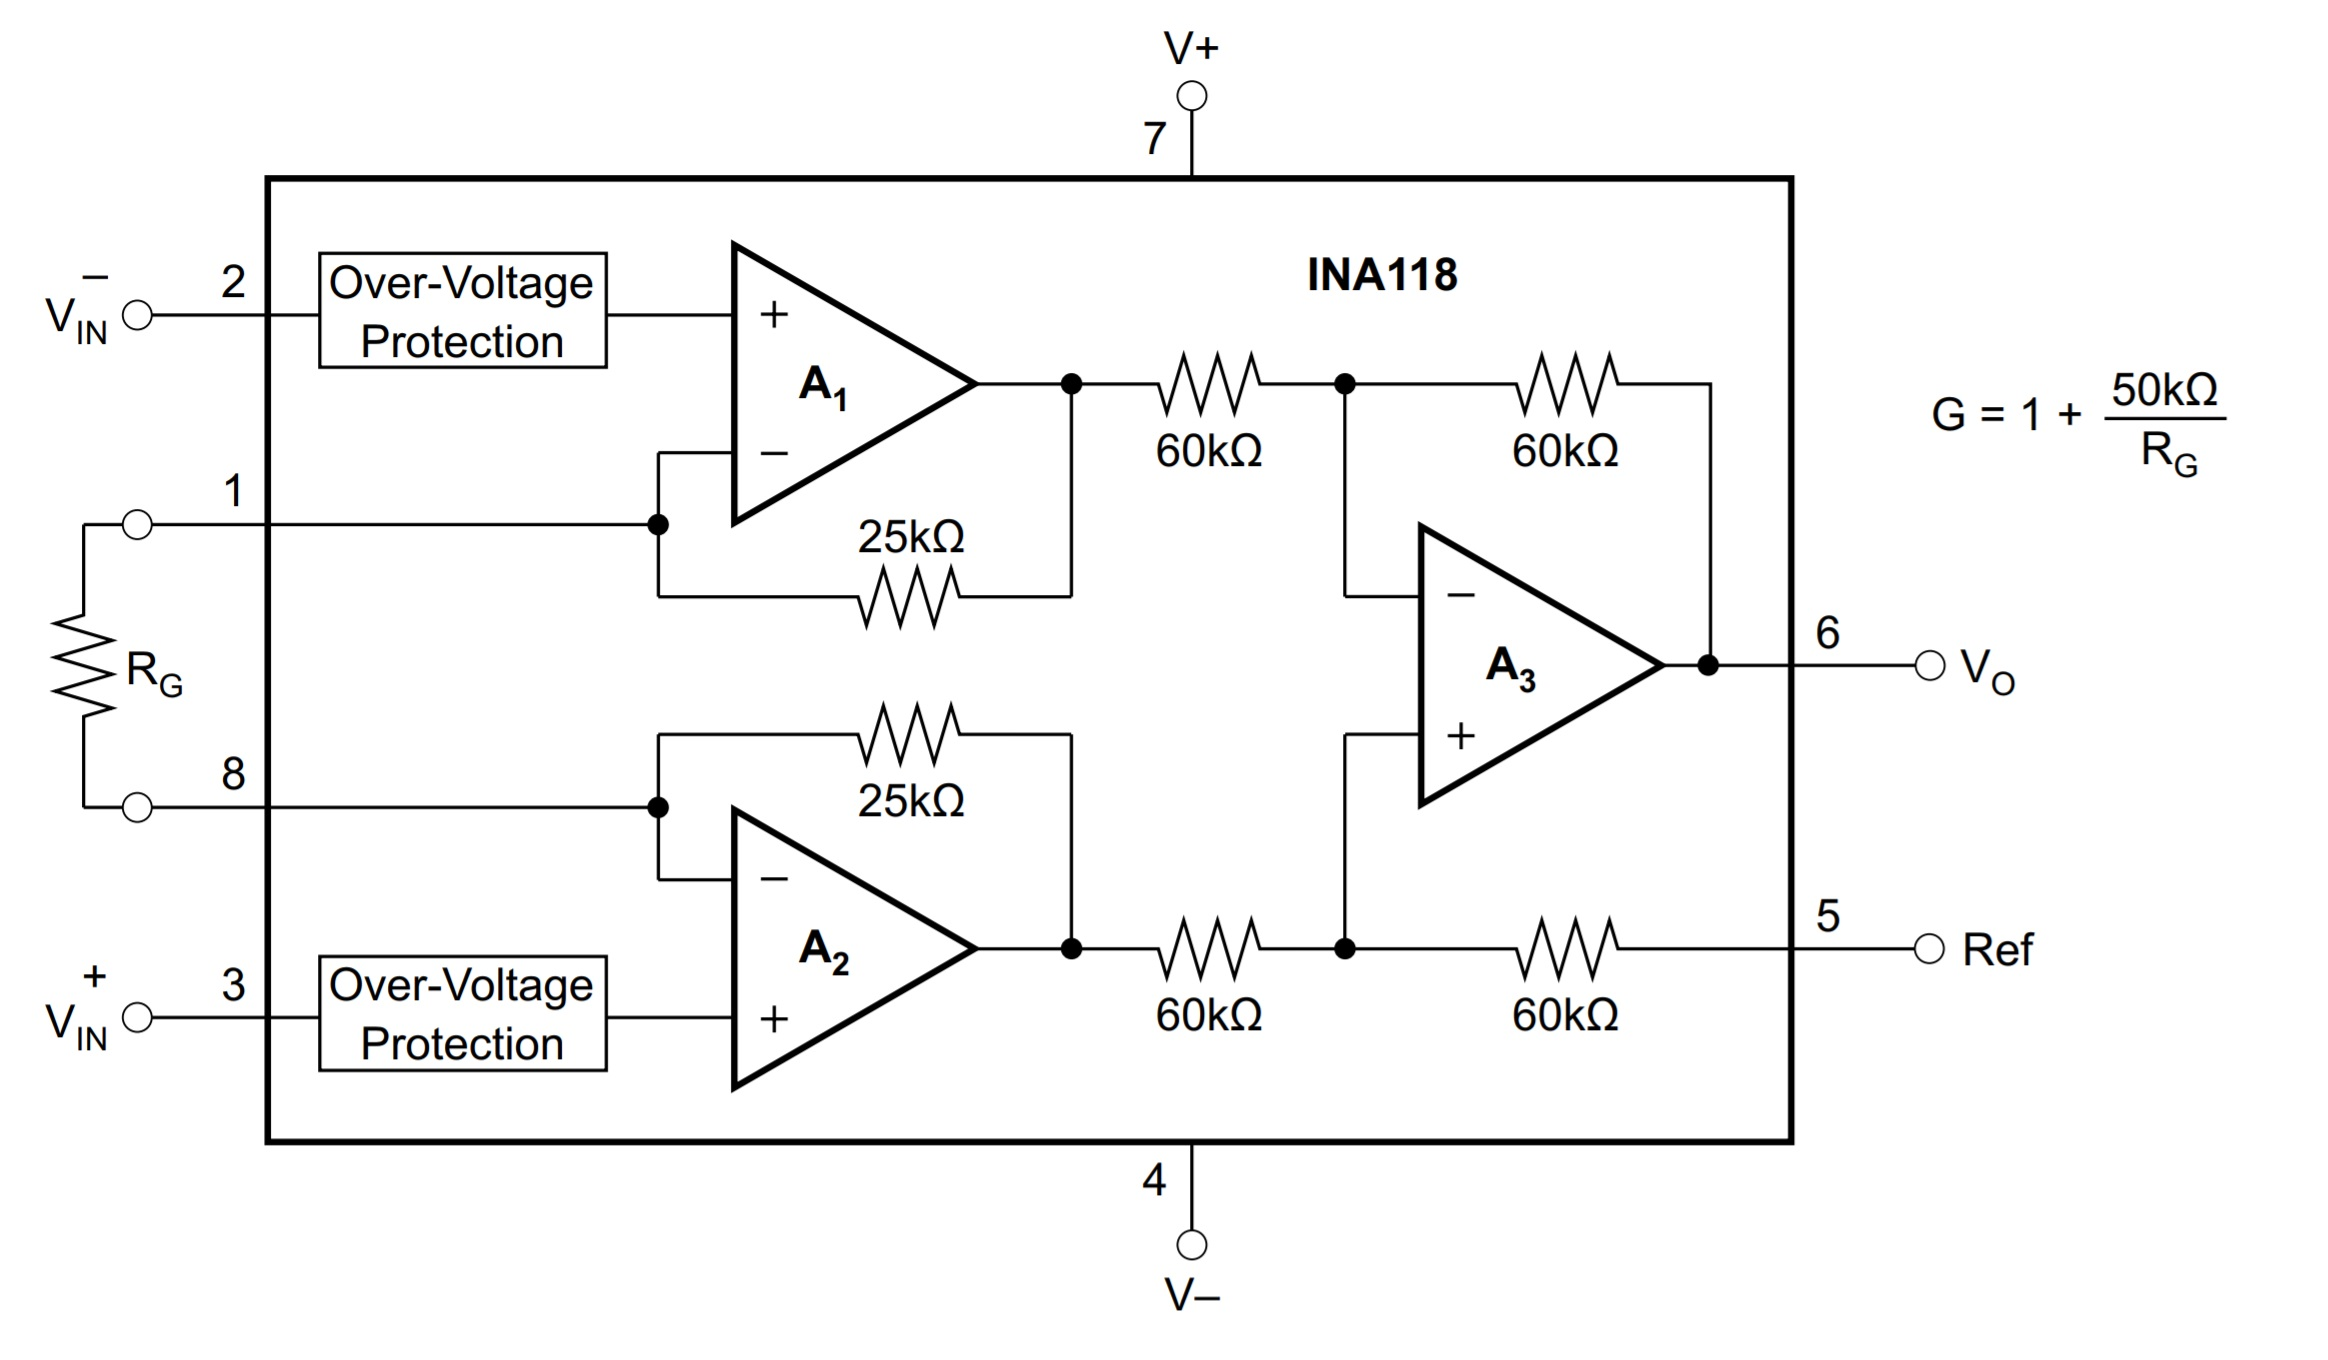
\includegraphics[scale=1.4]{figuras/fig-ina118}
		\caption{INA 118 \cite{schematic-ina118}}
		\label{fig:ina118}
	\end{figure}

	\subsubsection{Important features to consider in a amplifier}\label{sssec:important-features-to-consider-in-a-amplifier}

		There are some important factors when choosing a OPAMP in a certain application, according to \cite{analog2011operational}, some of the important features to know in a amplifier are:

		\begin{itemize}
			\item\textit{\textit{Common-Mode Voltage Range (CMVR):}} Allowable input voltage range at both inputs before clipping or excessive nonlinearity.\label{itm:opamp-cmrr}
			\item\textit{\textit{Common-Mode Rejection Ratio (CMRR):}} The ratio of common-mode voltage range (CMVR) to the change in the input offset voltage over this range, expressed in dB.\label{itm:opamp-cmrr}
			\item\textit{\textit{Gain Badwidth Product (GBW):}} The product of open-loop and bandwidth at a specific frequency.\label{itm:opamp-gbw}
			\item\textit{\textit{Input Bias Current ($I_{B}$):}} The current at the input terminals.\label{itm:opamp-input-bias-current}
			\item\textit{\textit{Operating Supply Voltage Range:}} The supply voltage range that can be applied to an amplifier for which it operates within specifications. Many applications implement op amp circuits with balanced dual supplies, while other applications for energy conservation or other reasons, use single-supply.\label{itm:opamp-operating-supply-voltage-range}
			\item\textit{\textit{Supply Current:}} The current required from the supply voltage to operate the amplifier with no load.\label{itm:opamp-supply-current}
		\end{itemize}